\documentclass{article}

\usepackage{multirow}
\usepackage[utf8]{inputenc}
\usepackage[bottom]{footmisc}
\usepackage{lscape}
\usepackage{pdfpages}
\setboolean{@twoside}{false}
\usepackage{graphicx}
\usepackage{epstopdf}
\usepackage[left=3cm,top=3cm,right=2cm,bottom=2cm]{geometry}%esq e sup 3cm  ; dir e inf 2cm
\usepackage[hang,small,bf]{caption}
\usepackage[compact]{titlesec}
\usepackage{etoolbox}
\usepackage{setspace}
\usepackage{amsthm}
\usepackage[figuresright]{rotating}
\usepackage{float}
\usepackage{amssymb}
\usepackage{graphicx}
\usepackage{fancybox}
\usepackage{amsmath}
\usepackage{enumitem}
\usepackage{picinpar}
\usepackage[toc,title]{appendix}
\usepackage{colortbl}
\usepackage{wasysym}
\usepackage{txfonts}
\usepackage{pb-diagram}
\usepackage{relsize}
\usepackage{tikz}
\usepackage{pgfplots}
\usepackage{subfigure}
\usepackage{lscape}
\usepackage{tabularx}
\usepackage{csquotes}
\usepackage{tocloft}
\renewcommand{\tablename}{Tabela}
\def\baselinestretch{1.5}
\pagestyle{myheadings}
\begin{document}
\titlespacing{\section}{0cm}{1.5cm}{1.5cm}
\titlespacing{\subsection}{0cm}{1.5cm}{1.5cm}
\label{pagina-de-rosto}
\pagestyle{empty}
\begin{tabular}{p{430pt}}
  \pagestyle{empty}
  \begin{center}
    %\pagestyle{empty}
    \Large{\begin{center}Luiz Gustavo Caobianco\end{center}}\bigskip \bigskip \bigskip \bigskip \bigskip \bigskip \bigskip \bigskip \bigskip \bigskip \bigskip \bigskip \bigskip \bigskip\bigskip \bigskip \bigskip  \bigskip \textbf{\LARGE{Implementa\c{c}\~{a}o da Rede Perceptron na Linguagem Java}}
  \end{center}
  \vspace*{+30pt}
  \hspace*{+200pt}
  \begin{tabular}{p{200pt}}
    \singlespacing{\small Exercício Para Casa - EPC01, da disciplina Redes Neurais Artificiais. \bigskip \bigskip \bigskip  \bigskip  Docente: Prof. Dr. Ivan Nunes} \\
  \end{tabular}
  \newline
  \newline
  \newline
  \newline
  \newline
  \bigskip
  \bigskip
  \bigskip \bigskip
  \bigskip \bigskip
  \newline
  \begin{center}
    {\large S\~{a}o Carlos - SP \\ Data de entrega: 03 de abril de 2018}
  \end{center}
\end{tabular}

\clearpage
\mainmatter
\section{Discussão  do Conjunto de Entrada}
\label{sec:discussao_entrada}
\hspace*{15pt} O conjunto de dados fornecido na proposta impedia a convergência do software implementado em linguagem Java. Estes dados foram testados com a toolbox do MATLAB e este por sua vez também não apresentou convergência para a solução.

\par É possível que o problema dado seja não linearmente separável. Entretanto, para a demonstração do método desenvolvido, bem como para o preenchimento da tabela apresentada na proposta, o conjunto de dados de entrada foi alterado, de modo que fosse possível converger.

\par Na tabela 1, é possível ver os valores que foram necessários serem modificados para permitir a convergência do método. Os valores da coluna \emph{d} em vermelho foram os valores que sofreram modificações. Se no conjunto de dados original um destes valores era 1, foi necessário a mudança para -1. Caso o valor original fosse -1, a mudança feita foi para 1.

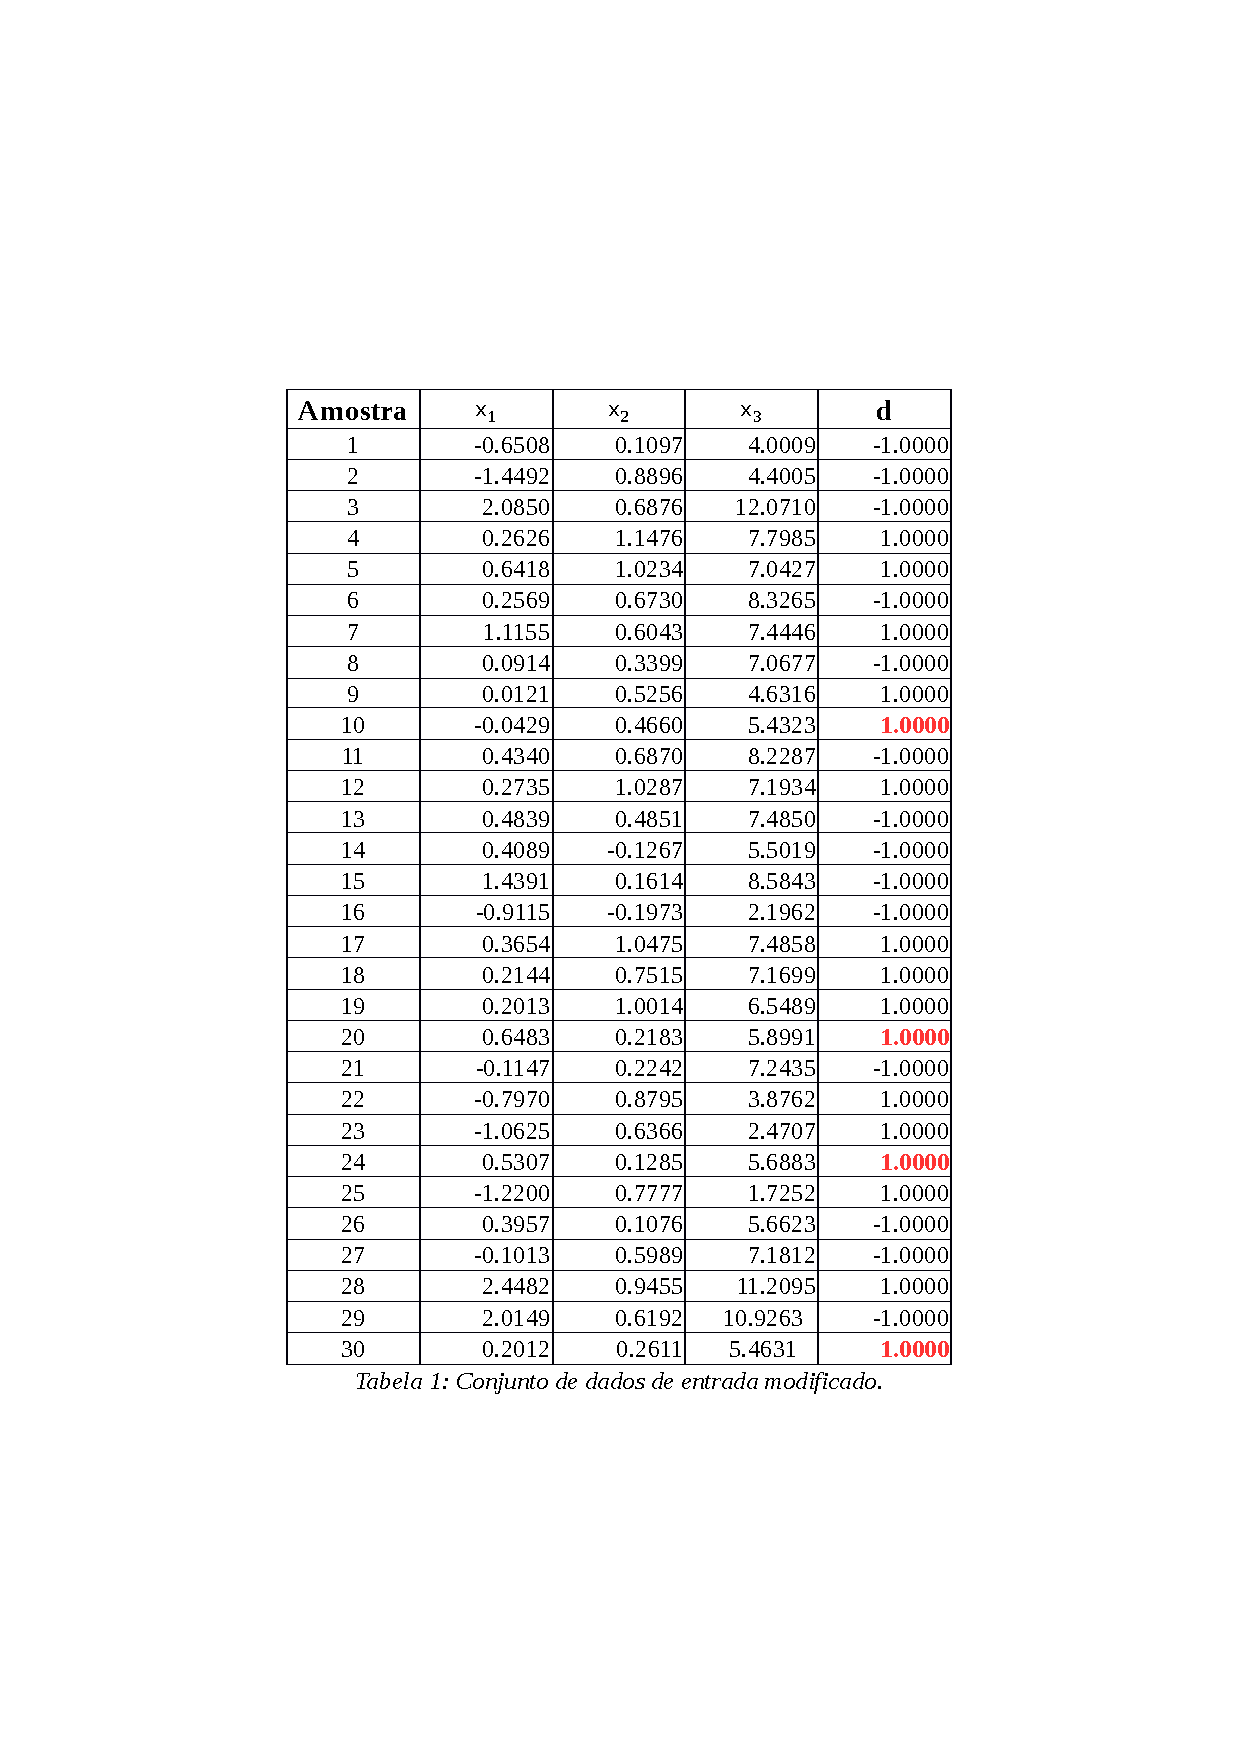
\includepdf[pages=-]{dados_entrada_modificados.pdf}



\section{Fase de Treinamento}
\label{sec:fase_treinamento}
\par Com o processo discutido na seção \ref{sec:discussao_entrada}, o software foi capaz de convergir e encontrar os resultados mostrados na tabela 2. Os números iniciais foram gerados novamente para cada treinameto.

\begin{landscape}
\begin{table}
\renewcommand\thetable{2}
\centering
\begin{tabular}{llllllllll}
\hline
\multicolumn{1}{|c|}{\multirow{2}{*}{Treinamento}} & \multicolumn{4}{l|}{Vetor de Pesos Inicial} & \multicolumn{4}{l|}{Vetor de Pesos Final} & \multicolumn{1}{l|}{\multirow{2}{*}{Núm. de Épocas}} \\ \cline{2-9}
 \multicolumn{1}{|c|}{} & \multicolumn{1}{l|}{w_0} & \multicolumn{1}{l|}{w_1} & \multicolumn{1}{l|}{w_2} & \multicolumn{1}{l|}{w_3} & \multicolumn{1}{l|}{w_0} & \multicolumn{1}{l|}{w_1} & \multicolumn{1}{l|}{w_2} & \multicolumn{1}{l|}{w_3} & \multicolumn{1}{l|}{} \\ \hline\multicolumn{1}{|l|}{1} &\multicolumn{1}{|l|}{-1} & \multicolumn{1}{|l|}{0,0229} & \multicolumn{1}{|l|}{0,8063} & \multicolumn{1}{|l|}{0,8226} & \multicolumn{1}{|l|}{1,4835} & \multicolumn{1}{|l|}{4,944} & \multicolumn{1}{|l|}{-0,5562} & \multicolumn{1}{|l|}{54,0226} & \multicolumn{1}{l|} {2660}\\\hline
\multicolumn{1}{|l|}{2} &\multicolumn{1}{|l|}{-1} & \multicolumn{1}{|l|}{0,3129} & \multicolumn{1}{|l|}{0,3188} & \multicolumn{1}{|l|}{0,5744} & \multicolumn{1}{|l|}{1,4865} & \multicolumn{1}{|l|}{4,9359} & \multicolumn{1}{|l|}{-0,5564} & \multicolumn{1}{|l|}{52,8744} & \multicolumn{1}{l|} {2615}\\\hline
\multicolumn{1}{|l|}{3} &\multicolumn{1}{|l|}{-1} & \multicolumn{1}{|l|}{0,4178} & \multicolumn{1}{|l|}{0,2955} & \multicolumn{1}{|l|}{0,4094} & \multicolumn{1}{|l|}{1,4864} & \multicolumn{1}{|l|}{4,9298} & \multicolumn{1}{|l|}{-0,5558} & \multicolumn{1}{|l|}{52,5294} & \multicolumn{1}{l|} {2606}\\\hline
\multicolumn{1}{|l|}{4} &\multicolumn{1}{|l|}{-1} & \multicolumn{1}{|l|}{0,6045} & \multicolumn{1}{|l|}{0,588} & \multicolumn{1}{|l|}{0,5941} & \multicolumn{1}{|l|}{1,5058} & \multicolumn{1}{|l|}{4,9525} & \multicolumn{1}{|l|}{-0,561} & \multicolumn{1}{|l|}{52,0541} & \multicolumn{1}{l|} {2573}\\\hline
\multicolumn{1}{|l|}{5} &\multicolumn{1}{|l|}{-1} & \multicolumn{1}{|l|}{0,9607} & \multicolumn{1}{|l|}{0,775} & \multicolumn{1}{|l|}{0,5382} & \multicolumn{1}{|l|}{1,5022} & \multicolumn{1}{|l|}{4,9437} & \multicolumn{1}{|l|}{-0,56} & \multicolumn{1}{|l|}{50,8182} & \multicolumn{1}{l|} {2514}\\\hline
\end{tabular}
\caption{Tabela em \LaTeX{} gerada automaticamente pelo software em Java}
\label{table:saida_software}
\end{table}
\end{landscape}


\section{Classificação de Novas Amostras}
\par Através dos treinamentos mostrados na seção \ref{sec:fase_treinamento}, novas amostras foram expostas ao software, que apresentou a classificação conforme mostrado na tabela 3.
\begin{table}[]
  \renewcommand\thetable{3}
\centering
\begin{tabular}{c|c|c|c|c|c|c|c|c|}
\cline{2-9}
\multicolumn{1}{l|}{}                  & \multicolumn{3}{c|}{Conjunto de entrada} & \multicolumn{5}{c|}{Classifica\c{c}\~{a}o}                                                                             \\ \hline
\multicolumn{1}{|c|}{\textbf{Amostra}} & $x_1$        & $x_2$       & $x_3$      & T1                      & T2                      & T3                      & T4                      & T5                      \\ \hline
\multicolumn{1}{|c|}{1}                & -0.3565      & 0.0620       & 5.9891     & -1                      & -1                      & -1                      & -1                      & -1                      \\ \hline
\multicolumn{1}{|c|}{2}                & -0.7842      & 1.1267       & 5.5912     & 1                       & 1                       & 1                       & 1                       & 1                       \\ \hline
\multicolumn{1}{|c|}{3}                & 0.3012       & 0.5611       & 5.8234     & -1                      & -1                      & -1                      & -1                      & -1                      \\ \hline
\multicolumn{1}{|c|}{4}                & 0.7757       & 1.0648       & 8.0677     & 1                       & 1                       & 1                       & 1                       & 1                       \\ \hline
\multicolumn{1}{|c|}{5}                & 0.1570       & 0.8028       & 6.3040     & 1                       & 1                       & 1                       & 1                       & 1                       \\ \hline
\multicolumn{1}{|c|}{6}                & -0.7014      & 1.0316       & 3.6005     & 1                       & 1                       & 1                       & 1                       & 1                       \\ \hline
\multicolumn{1}{|c|}{7}                & 0.3748       & 0.1536       & 6.1537     & -1                      & -1                      & -1                      & -1                      & -1                      \\ \hline
\multicolumn{1}{|c|}{8}                & -0.6920      & 0.9404       & 4.4058     & 1                       & 1                       & 1                       & 1                       & 1                       \\ \hline
\multicolumn{1}{|c|}{9}                & -1.3970      & 0.7141       & 4.9263     & -1                      & -1                      & -1                      & -1                      & -1                      \\ \hline
\multicolumn{1}{|c|}{10}               & -1.8842      & -0.2805      & 1.2548     & \multicolumn{1}{l|}{-1} & \multicolumn{1}{l|}{-1} & \multicolumn{1}{l|}{-1} & \multicolumn{1}{l|}{-1} & \multicolumn{1}{l|}{-1} \\ \hline
\end{tabular}
\caption{Resposta do Software}
\end{table}

\section{Variação do Número de Épocas}
\hspace*{15pt} Os vetores de pesos iniciais são gerados aleatoriamente, e conforme a rede é treinada, estes valores convergem na direção da solução correta, desde que o conjunto de entrada seja linearmente separável. Isto significa que, uma vez que sorteados, estes valores são alterados até a solução do problema.

\par A variação do número de épocas deve-se exatamente ao sorteio inicial. Se, por coincidência, os números gerados aleatoriamente forem próximos da solução inicial, será necessário uma quantidade menor de épocas  para encontrar a solução do sistema.

\par Analogamente, se os números sorteados forem distantes dos números que representam uma solução para o problema, será necessário uma quantidade maior de épocas para que seja encontrado o resultado.

\section{A limitação da Perceptron}
\hspace*{15pt} A principal limitação deve-se ao fato que só é possível resolver problemas linearmente separáveis. Isso significa que, conforme aumentamos a quantidade de entradas, a solução apresentada pela Perceptron perde a precisão.

\par Por exemeplo, com apenas duas entradas, um problema linearmente separável pode ser isolado por uma simples reta, e neste caso a Perceptron apresenta ótimo desempenho. Entretanto, caso seja necessário utilizar 3, 4, ou mais entradas, a solução apresentada pela Perceptron não será tão precisa quanto uma rede Perceptron de duas entradas.

\newpage
\section{Anexos}
\par Nesta seção, os códigos em Java da implementação feita são demonstrados. Os códigos foram impressos através da funcionalidade embutida de impressão de código da IDE IntelliJ Ultimate, registrado no nome do autor deste trabalho.

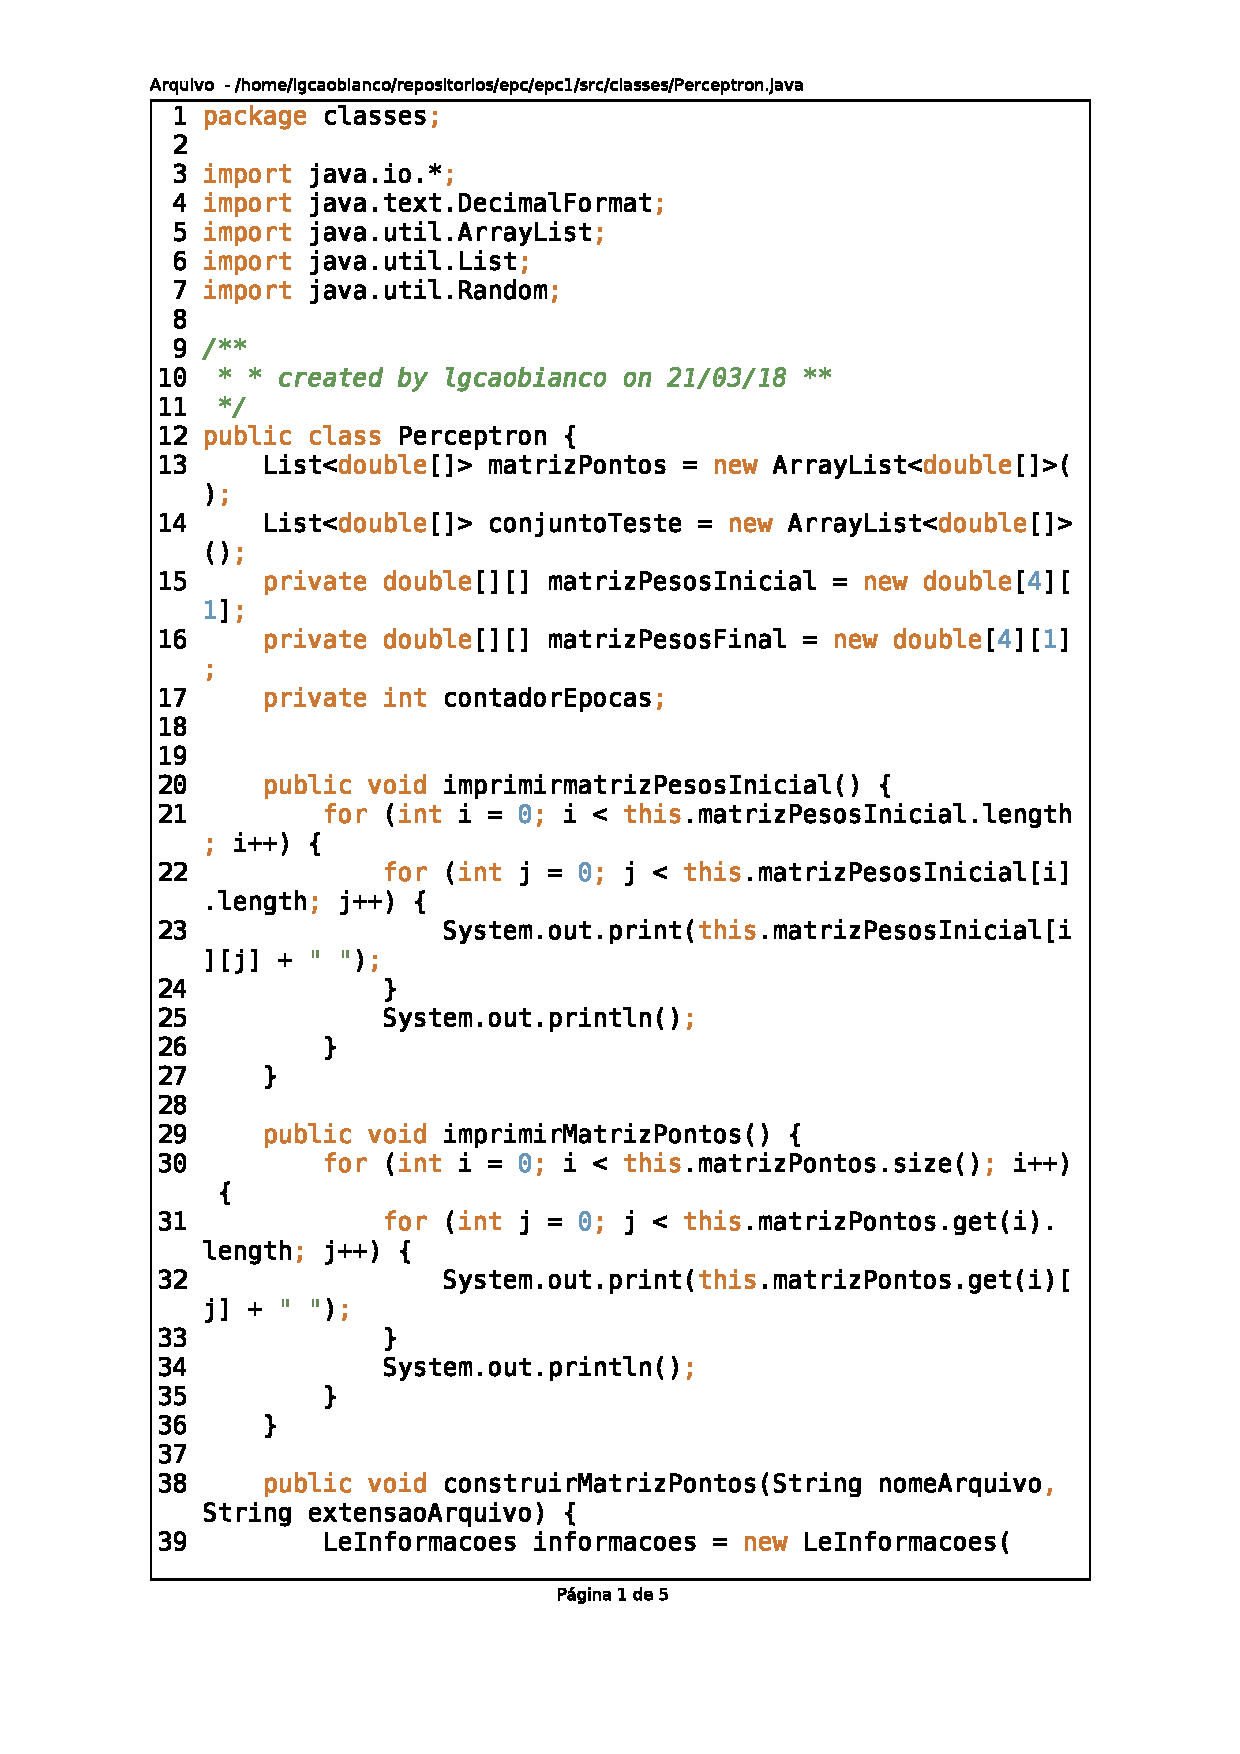
\includepdf[pages=-,pagecommand={}]{codigo_classe_base.pdf}
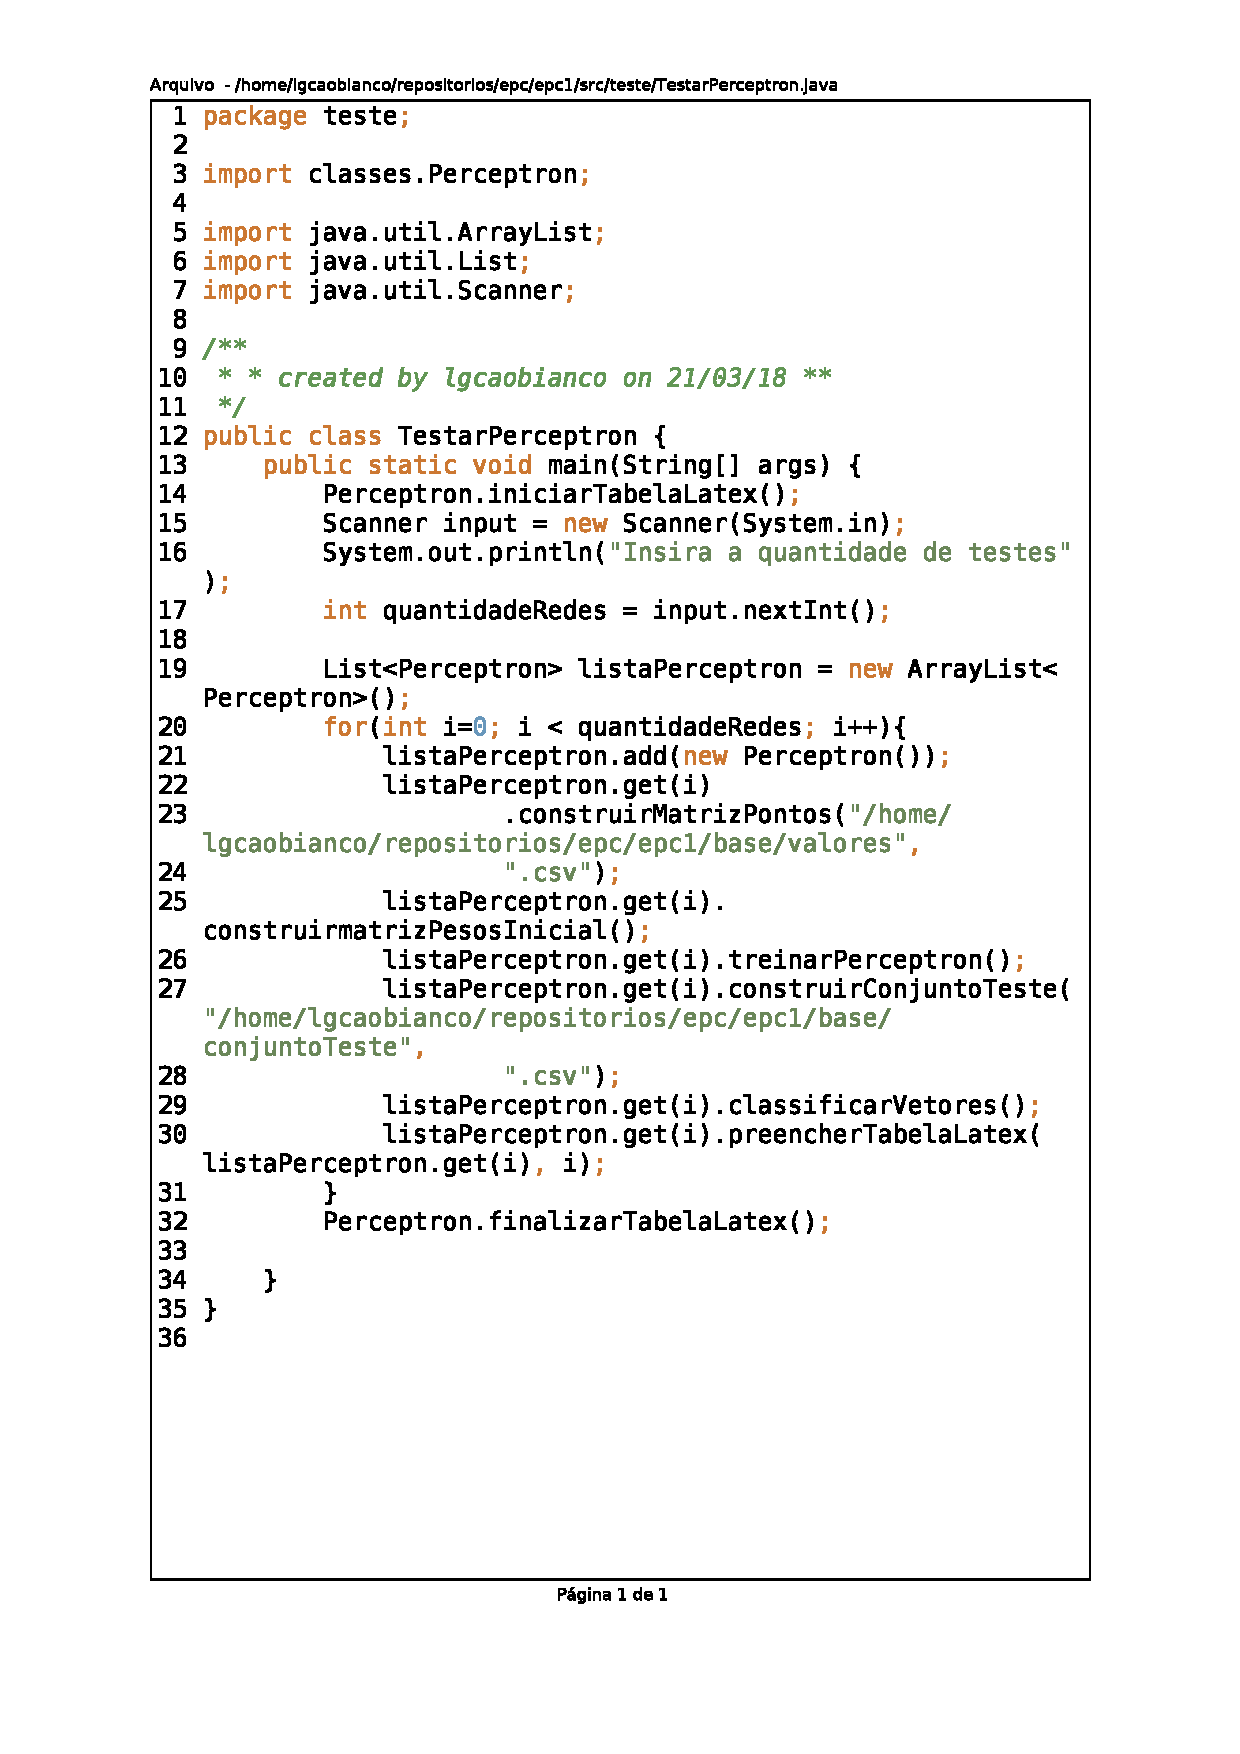
\includepdf[pages=-,pagecommand={}]{codigo_classe_teste.pdf}


\end{document}
